\subsubsection{La vue}
\label{subsubsec:sonVue}

Pour pouvoir se déplacer dans le labyrinthe, l'existence de fichiers audios
stockant nos voix est nécessaire. Et pour permettre à n'importe quel
utilisateur de pouvoir créer ses propres fichiers audios, il faut qu'il y ait
une interface graphique qui lui facilite la tâche.

On note ainsi les deux points clés essentiels que doit pouvoir faire un
utilisateur:
\begin{itemize}
    \item{\makebox[2cm][l]{\texttt{Ajouter}}     / \makebox[1.5cm][l]{\texttt{Modifier}} / \makebox[2cm][l]{\texttt{Supprimer}} un joueur.}
    \item{\makebox[2cm][l]{\texttt{Enregistrer}} / \makebox[1.5cm][l]{\texttt{Écouter}}  / \makebox[2cm][l]{\texttt{Supprimer}} un audio.}
\end{itemize}

\subsubsection*{Le Menu Audio}
\label{subsubsec:AudioMenu}

Le menu audio est la première interface graphique que l'utilisateur voit
lorsqu'il se rend dans les paramètres du jeu. Il permet de gérer la
quasi-totalité des besoins précédemment énoncés, et envoie vers les pages
qui gèrent les autres.
La classe \textbf{\textit{AudioMenu}} tient les ficelles de ce menu.

\begin{figure}[!htb]
    \centering
    % TODO: @GitFenixZ | Update captions
    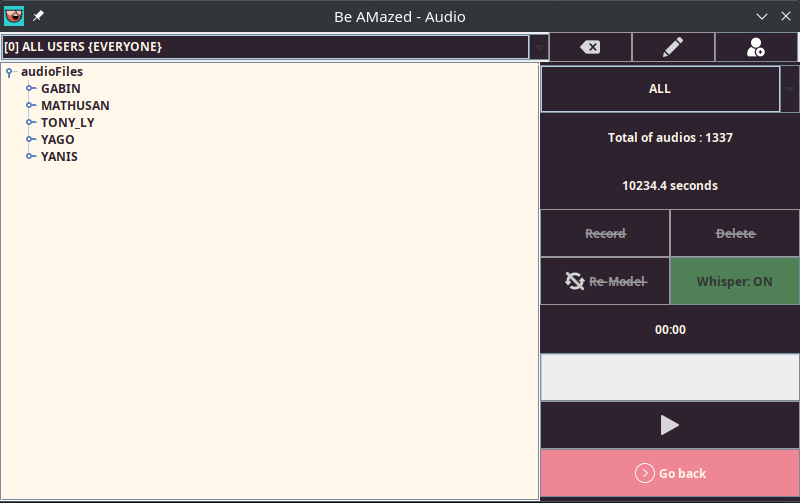
\includegraphics[width=8cm]{ressources/Implementation/Son/AudioMenu.png}%
    \caption{Image du menu Audio}%
    \label{fig:AudioMenu}
\end{figure}

De là, on remarque que le menu est divisé en trois parties.
Le centre de l'écran qui représente l'arborescence des fichiers audios
(\ref{fig:audioFilesTree}).
Puis sur la partie supérieure de l'écran, on retrouve les boutons qui
permettent la gestion des utilisateurs.
Enfin, sur la droite de l'écran, on retrouve les boutons qui permettent une vue
globale et une gestion des fichiers audios.

\paragraph{L'arborescence des fichiers audios}

L'arborescence des fichiers audios est représentée par un objet de la classe
\textbf{\textit{FileTree}} qui étend la classe \textbf{\textit{JTree}} de Java.
Elle permet une personnalisation accrue de l'arborescence, notamment en
permettant de changer la couleur des noeuds, ou encore de changer l'icône des
noeuds feuilles. De plus, à l'aide d'une \texttt{regex}, nous avons pu afficher
uniquement les fichiers audios qui intéressent l'utilisateur.

\paragraph{La gestion des utilisateurs}
Cette partie du menu se décompose en quatre éléments
\begin{itemize}
    \item{Séléction des utilisateurs dans la liste}
    \item{Ajouter un utilisateur}
    \vcenteredinclude[height=5mm]{ressources/Implementation/Son/add-user.png}
    \item{Modifier un utilisateur}
    \vcenteredinclude[height=5mm]{ressources/Implementation/Son/edit.png}
    \item{Supprimer un utilisateur}
    \vcenteredinclude[height=5mm]{ressources/Implementation/Son/delete-button.png}
\end{itemize}

\paragraph{La gestion des fichiers audios}

Sans compter le bouton de retour au menu principal, cette partie du menu se
décompose en 8 éléments

\begin{enumerate}
    \item{Le choix du mot}
    \item{Le nombre d'audios enregistrés}
    \item{La durée totale déjà enregistrée}
    \item{Un bouton d'enregistrement} (\ref{subsubsec:sonVueEnregistrementAudio})
    \item{Un bouton de suppression}
    \item{Un bouton de modélisation}
    \item{Un bouton ON/OFF concernant l'utilisation de whisper}
    \item{Un timer}
    \item{Une barre de progression}
    \item{Un bouton d'écoute}
\end{enumerate}

\begin{figure}[htb]
    \centering
    % TODO: @GitFenixZ | Update captions
    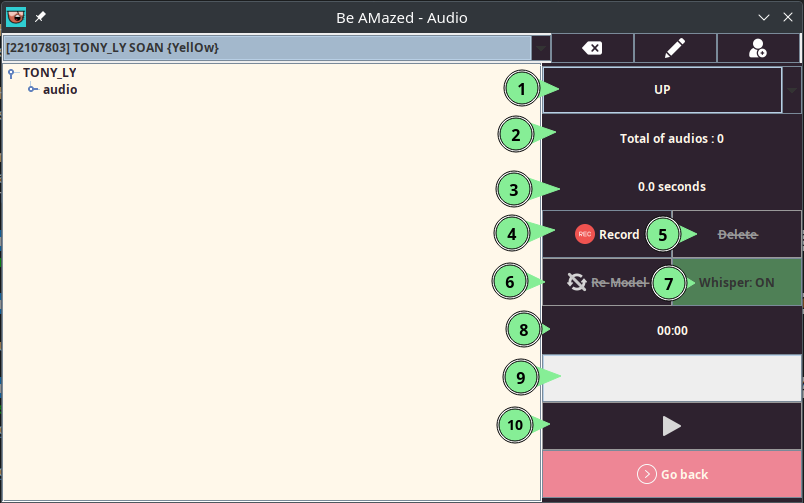
\includegraphics[width=8cm]{ressources/Implementation/Son/GestionFichiersAudio.png}%
    \caption{Image de l'interaction avec les fichiers audios}%
\end{figure}

Le choix du mot est un élément qui permet de choisir le mot que l'on souhaite
enregistrer. Il est composé d'une liste déroulante qui contient tous les mots
disponibles dans le jeu (Voir la classe \textbf{\textit{WordToRecord}}) et en
y ajoutant le mot global \texttt{ALL}.
Lorsqu'un mot est sélectionné, le nombre d'audios enregistrés et la durée
totale sont mis à jour en fonction du mot choisi et du joueur sélectionné.

Lorsque un audio est sélectionné, les boutons de suppression et d'écoute
s'activent. Si le bouton d'écoute est cliqué, alors l'audio est joué et au
la barre de progression et le timer sont mis à jour en temps réel en fonction
de la durée de l'audio.

Si le bouton de suppression est cliqué, alors l'audio est supprimé et l'arborescence
est mise à jour.

Et pour pouvoir cliquer sur le bouton \texttt{Record}, il est nécessaire que le
joueur et le mot aient été choisis.


\subsubsection*{La page d'ajout/de modification d'un utilisateur}
\label{subsubsec:sonVueAjoutModifUtilisateur}

Les pages de création et de modification de l'utilisateur sont identiques, à
l'exception du bouton de validation qui est respectivement \texttt{Create}
et \texttt{Save}. La classe \textbf{\textit{EditCreateUsersPage}} gère ces
pages.

\begin{figure}[!htb]
    \centering
    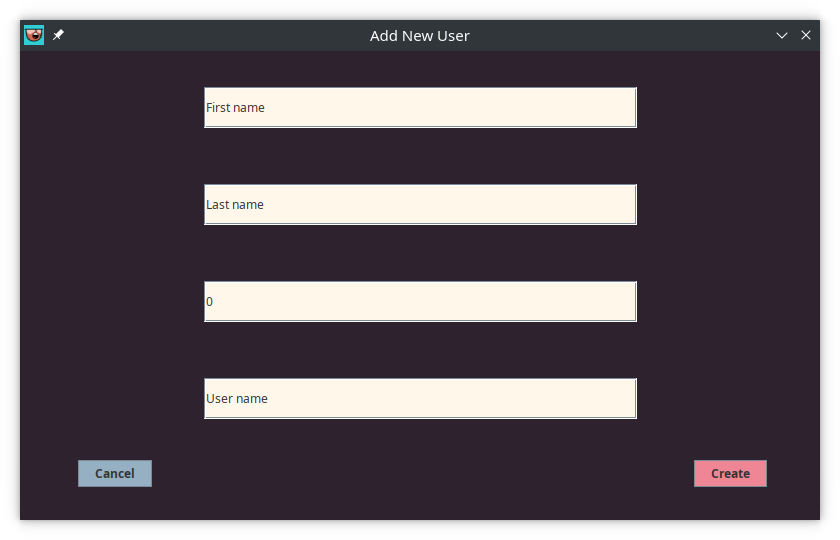
\includegraphics[width=8cm]{ressources/Implementation/Son/AddEditUser.png}%
    \caption{Image de la page d'ajout/de modification d'un utilisateur}
    \label{fig:CreateOrSaveUserPage}
\end{figure}

\subsubsection*{La page d'enregistrement d'un audio}
\label{subsubsec:sonVueEnregistrementAudio}

La page d'enregistrement permet d'enregistrer des audios pour un mot et un joueur
donné. La classe \textbf{\textit{RecordPage}} gère cette page. On y retrouve un
timer, le nombre d'audios enregistrés depuis le début de la "session", un bouton
d'enregistrement \texttt{Record}, un bouton \texttt{Discard}, un bouton
\texttt{Discard All} et un bouton de retour au menu audio.
Lorsque le bouton \texttt{Record} est cliqué, l'enregistrement commence, le countdown
du timer commence et le bouton \texttt{Record} devient \texttt{Stop}. L'enregistrement
s'arrête lorsque le bouton \texttt{Stop} est cliqué ou lorsque le décompte se termine.
Si le bouton \texttt{Discard} est cliqué pendant que l'enregistrement est en cours,
alors ce dernier se stoppe et l'audio est supprimé, sinon le dernier audio est
directement supprimé.
Si le bouton \texttt{Discard All} est cliqué, alors tous les audios enregistrés
depuis le début de la "session" sont supprimés après confirmation de l'utilisateur.

\begin{figure}[!htb]
    \centering
    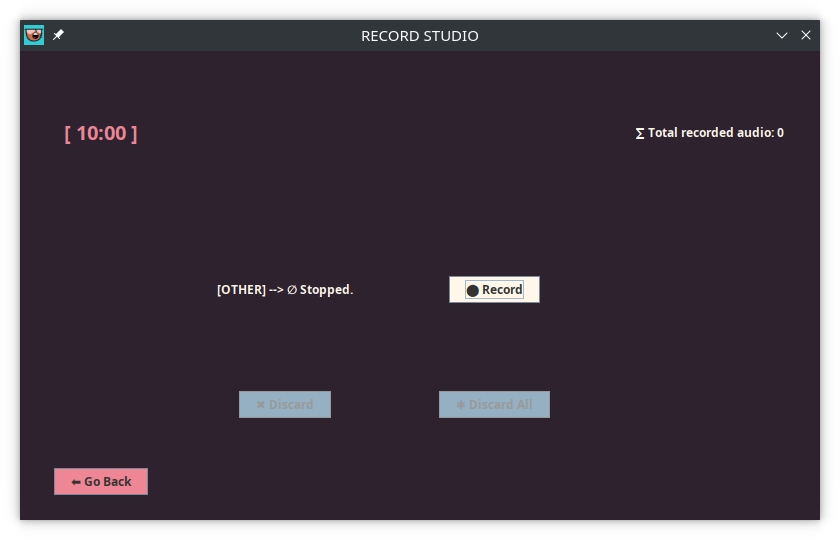
\includegraphics[width=8cm]{ressources/Implementation/Son/RecordPage.png}%
    \caption{Image de la page d'enregistrement}
    \label{fig:RecordPage}
\end{figure}
